\section{Nonlinear Optimization}

In this section we discuss the generic nonlinear optimization problem that forms the basis for the rest of the material presented in this class. We write the minimization problem as 
\begin{equation*}
\begin{aligned}
& \underset{\bm{x} \in \mathcal{X}}{\min}
& & f(\bm{x})
\end{aligned}
\end{equation*}
where $f$ is the cost function, usually assumed twice continuously differentiable, $x \in \R^n$ is the optimization variable, and $\mathcal{X} \subset \R^n$ is the constraint set. The special case in which the cost function is linear and the constraint set is specified by linear equations and/or inequalities is \textit{linear optimization}, which we will not discuss. 

\subsection{Unconstrained Nonlinear Optimization}

We will first address the unconstrained case, in which $\mathcal{X} = \R^n$. A vector $\bm{x}^*$ is said to be an unconstrained \textit{local minimum} if there exists $\epsilon > 0$ such that $f(\bm{x}^*) \leq f(\bm{x})$ for all $\bm{x} \in \{\bm{x} \mid \|\bm{x} - \bm{x}^*\| \leq \epsilon\}$, and $\bm{x}^*$ is said to be an unconstrained \textit{global minimum} if $f(\bm{x}^*) \leq f(\bm{x})$ for all $x \in \R^n$. 

\subsubsection{Necessary Conditions for Optimality}

For a differentiable cost function, we can compare the cost of a point to its neighbors by considering a small variation $\Delta \bm{x}$ from $\bm{x}^*$. By using Taylor expansions, this yields a first order cost variation
\begin{equation}
    f(\bm{x}^* + \Delta \bm{x}) - f(\bm{x}^*) \approx \nabla f(\bm{x}^*)^T \Delta \bm{x}
\end{equation}
and a second order cost variation 
\begin{equation}
    f(\bm{x}^* + \Delta \bm{x}) - f(\bm{x}^*) \approx \nabla f(\bm{x}^*)^T \Delta \bm{x} + \frac{1}{2} \Delta \bm{x}^T \nabla^2 f(\bm{x}^*) \Delta \bm{x}.
\end{equation}
Setting $\Delta \bm{x}$ to be equal to positive and negative multiples of the unit coordinate vector, we have 
\begin{equation}
    \frac{\partial f(\bm{x}^*)}{\partial x_i} \geq 0
\end{equation}
where $x_i$ denotes the $i$'th coordinate of $\bm{x}$, and 
\begin{equation}
    \frac{\partial f(\bm{x}^*)}{\partial x_i} \leq 0
\end{equation}
for all $i$, which is only satisfied by $\nabla f(\bm{x}^*) = 0$.  This is referred to as the \textit{first order necessary condition for optimality}. Looking at the second order variation, and noting that $f(\bm{x}^*) = 0$, we expect
\begin{align}
f(\bm{x}^* + \Delta \bm{x}) - f(\bm{x}^*) \geq 0
\end{align}
and thus
\begin{align}
\Delta \bm{x}^T \nabla^2 f(\bm{x}^*) \Delta \bm{x} \geq 0
\end{align}
which implies $\nabla^2 f(\bm{x}^*)$ is positive semidefinite. This is referred to as the \textit{second order necessary condition for optimality}. Stating these conditons formally, 

\begin{theorem}[Necessary Conditions for Optimality (NOC)]
Let $\bm{x}^*$ be an unconstrained local minimum of $f:\R^n \to \R$ and $f \in C^1$ in an open set $S$ containing $\bm{x}^*$. Then,
\begin{equation}
    \nabla f(\bm{x}^*) = 0.
\end{equation}
If $f \in C^2$ within $S$, $\nabla^2 f(\bm{x}^*)$ is positive semidefinite. 
\end{theorem}

\proof{See section 1.1 of \cite{bertsekas2016nonlinear}}.

\subsubsection{Sufficient Conditions for Optimality}


\begin{figure}[t]
    \centering
    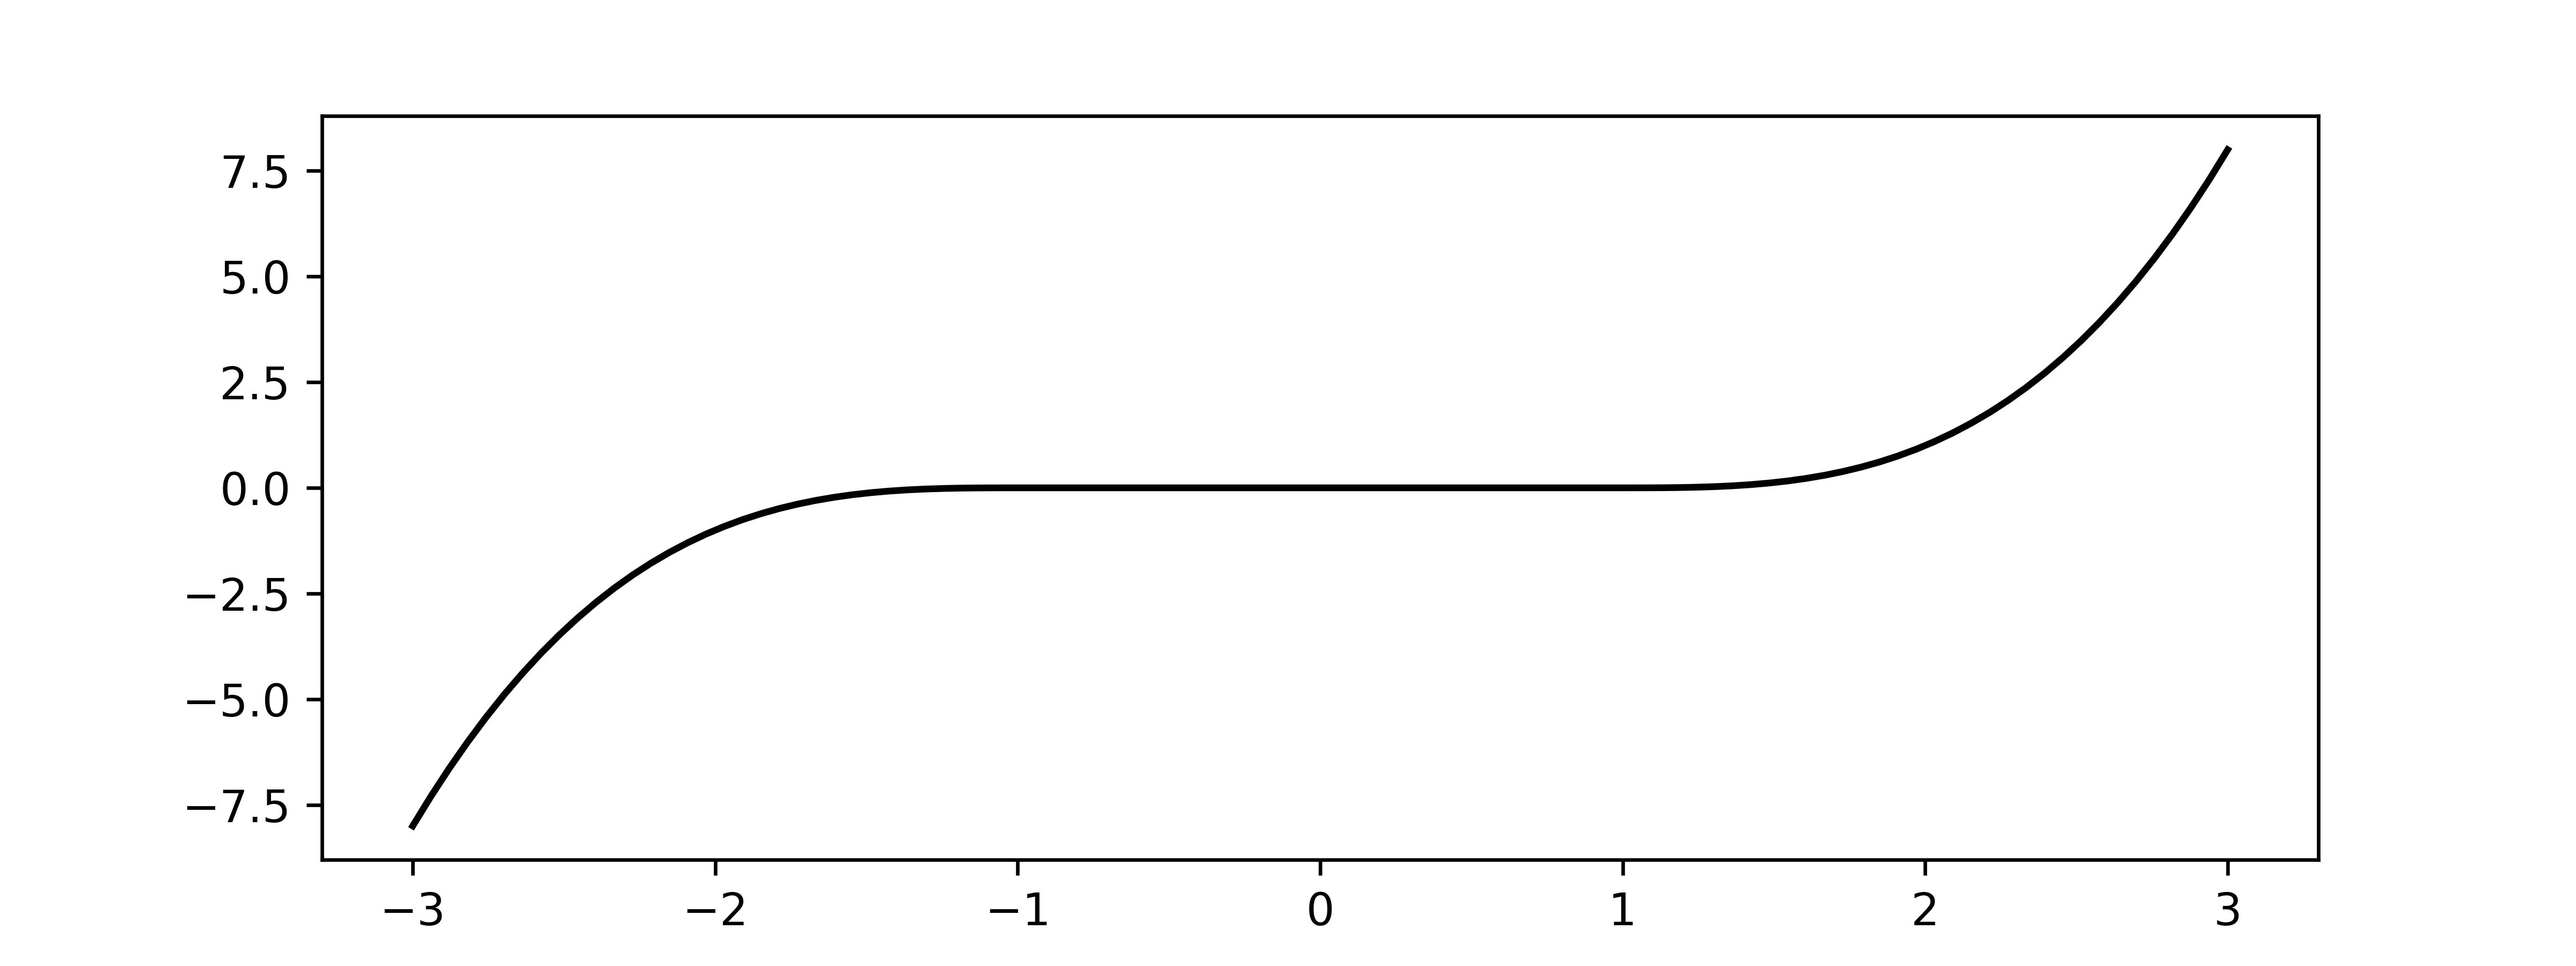
\includegraphics[width=0.7\linewidth]{figs/foc.png}
    \caption{An example of a function for which the necessary conditions of optimality are satisfied but the sufficient conditions are not.}
    \label{fig:foc}
\end{figure}


If we strengthen the second order condition to $\nabla^2 f(\bm{x}^*)$ being positive definite, we have the sufficient conditions for $\bm{x}^*$ being a local minimum. Why is the second order necessary conditions not sufficient? An example function is given in figure \ref{fig:foc}. Formally, 

\begin{theorem}[Sufficient Conditions for Optimality (SOC)]
Let $f:\R^n \to \R$ be $C^2$ in an open set $S$. Suppose a vector $\bm{x}^*$ satisfies the conditions $\nabla f(\bm{x}^*) = 0$ and $\nabla^2 f(\bm{x}^*)$ is positive definite. Then $\bm{x}^*$ is a strict unconstrained local minimum of $f$. 
\end{theorem}

Proof is again given in Section 1.1 of \cite{bertsekas2016nonlinear}.
There are several reasons why the optimality conditions are important. In a general nonlinear optimization setting, they can be used to filter candidates for global minima. They can be used for sensitivity analysis, in which the sensitivity of $\bm{x}^*$ to model parameters can be quantified \cite{bertsekas2016nonlinear}. This is common in e.g. microeconomics. Finally, these conditions often provide the basis for the design and analysis of optimization algorithms.

\subsubsection{Special case: Convex Optimization}

A special case within nonlinear optimization is the set of \textit{convex optimization} problems. A set $S \subset \R^n$ is called \textit{convex} if 
\begin{equation}
    \alpha \bm{x} + (1 - \alpha) \bm{y} \in S, \quad \forall \bm{x},\bm{y} \in S, \forall \alpha \in [0,1].
\end{equation}
For $S$ convex, a function $f:S\to\R$ is called convex if 
\begin{equation}
    f(\alpha \bm{x} + (1-\alpha) \bm{y}) \leq \alpha f(\bm{x}) + (1-\alpha) f(\bm{y}).
    \label{eq:conv_fun}
\end{equation}
This class of problems has several important characteristics. If $f$ is convex, then
\begin{itemize}
    \item A local minimum of $f$ over $S$ is also a global minimum over $S$. If in addition $f$ is strictly convex (the inequality in (\ref{eq:conv_fun}) is strict), there exists at most one global minimum of $f$.
    \item If $f \in C^1$ and convex, and the set $S$ is open, $\nabla f(\bm{x}^*) = 0$ is a necessary and sufficient condition for a vector $\bm{x}^* \in S$ to be a global minimum over $S$.
\end{itemize}
Convex optimization problems have several nice properties that make them (usually) computationally efficient to solve, and the first property above gives a certificate of having obtained global optimality that is difficult or impossible to obtain in the general nonlinear optimization setting. For a thorough treatment of convex optimization theory and algorithms, see \cite{boyd2004convex}. 

\subsubsection{Computational Methods}

In this subsection we will discuss the class of algorithms known as \textit{gradient methods} for finding local minima in nonlinear optimization problems. These approaches, rely (roughly) on following the gradient of the function ``downhill'', toward the minima. More concretely, these algorithms rely on taking steps of the form
\begin{equation}
    \bm{x}^{k+1} = \bm{x}^k + \alpha^{k} \bm{d}^k
\end{equation}
where if $\nabla f(\bm{x}) \neq 0$, $\bm{d}^k$ is chosen so that 
\begin{equation}
    \nabla f(\bm{x})^T \bm{d}^k < 0
\end{equation}
and $\alpha > 0$. Typically, the step size $\alpha^k$ is chosen such that 
\begin{equation}
    f(\bm{x}^k + \alpha^k \bm{d}^k) < f(\bm{x}^k),
\end{equation}
but generally, the step size and the direction of descent ($\bm{d}^k$) are tuning parameters. 

We will look at the general class of descent directions of the form 
\begin{equation}
    \bm{d}^k = -D^k \nabla f(\bm{x}^k)
\end{equation}
where $D^k > 0$ (note that this guarantees $\nabla f(\bm{x}^k)^T \bm{d}^k < 0$). 

\paragraph{Steepest descent, $D^k = I$.} The simplest choice of descent direction is directly following the gradient, and ignoring second order function information. In practice, this often leads to slow convergence (figure \ref{fig:graddesc_small}) and possible oscillation (figure \ref{fig:graddesc_large}).

\begin{figure}[!t]
    \centering
    \begin{subfigure}[b]{0.46\linewidth}
        \centering
        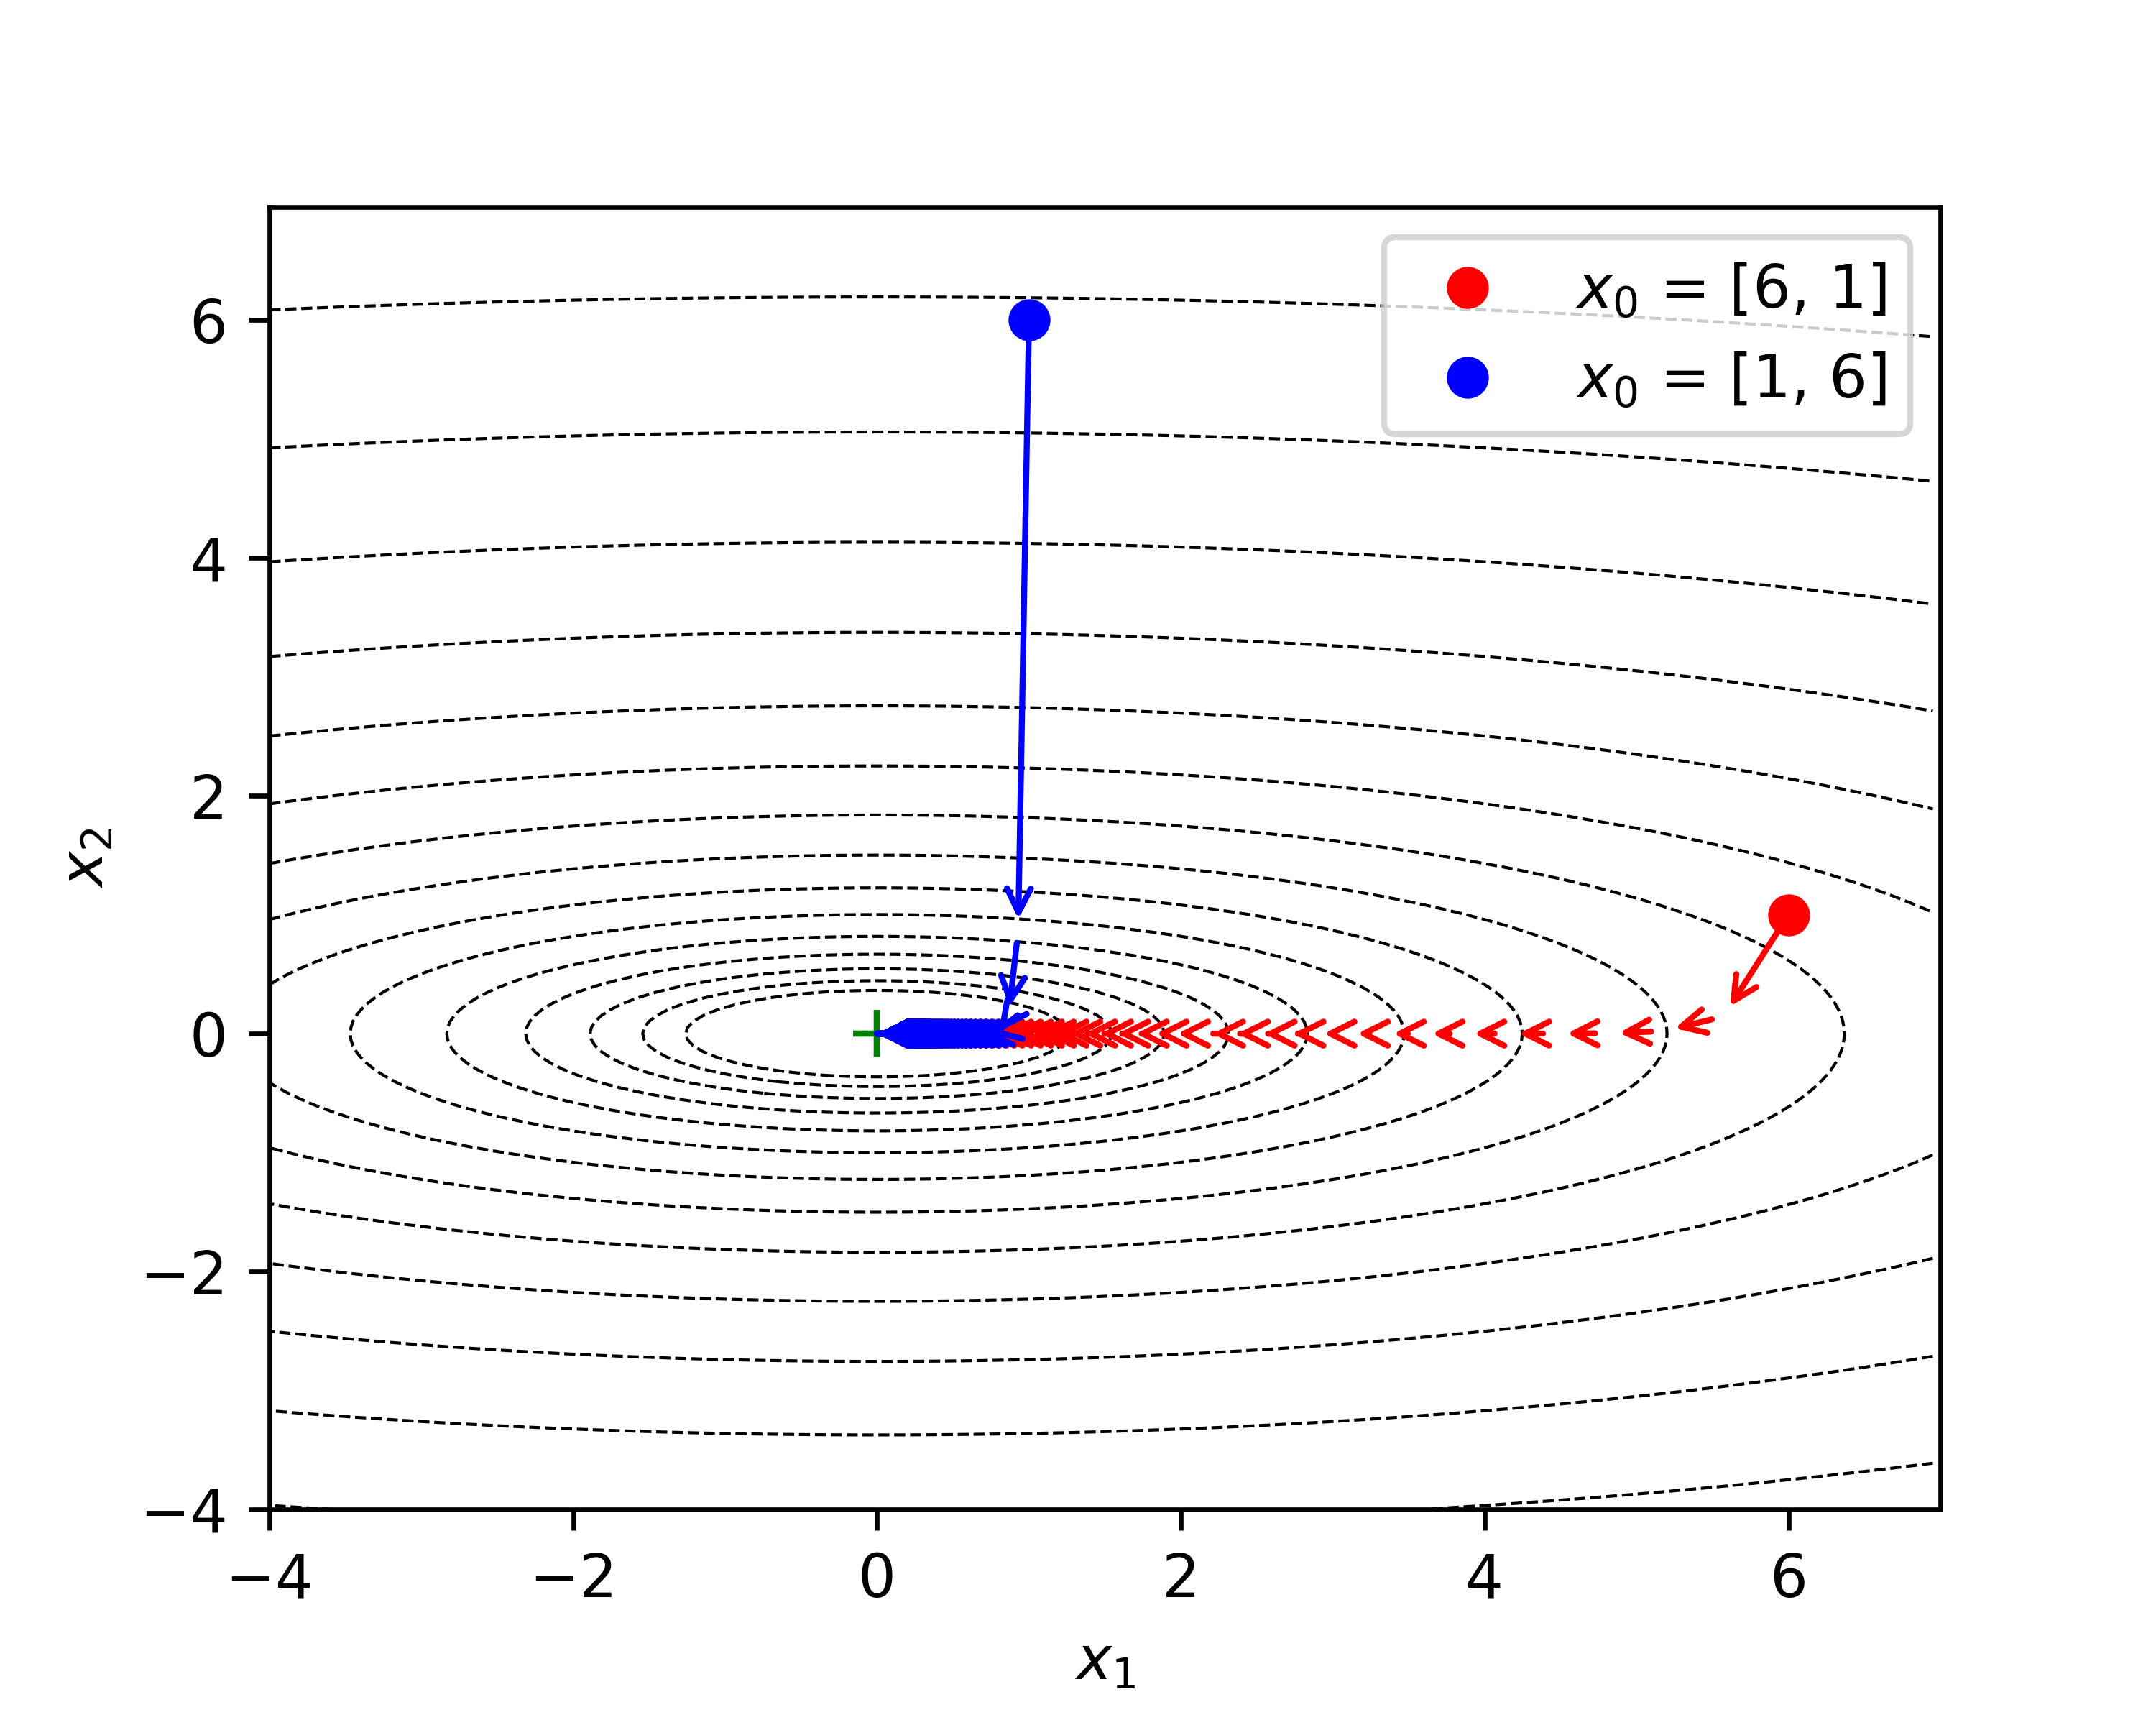
\includegraphics[width=\textwidth]{figs/small_step.png}
        \caption{Steepest descent, small fixed step size.}
        \label{fig:graddesc_small}
    \end{subfigure}%
    \begin{subfigure}[b]{0.46\linewidth}
        \centering
        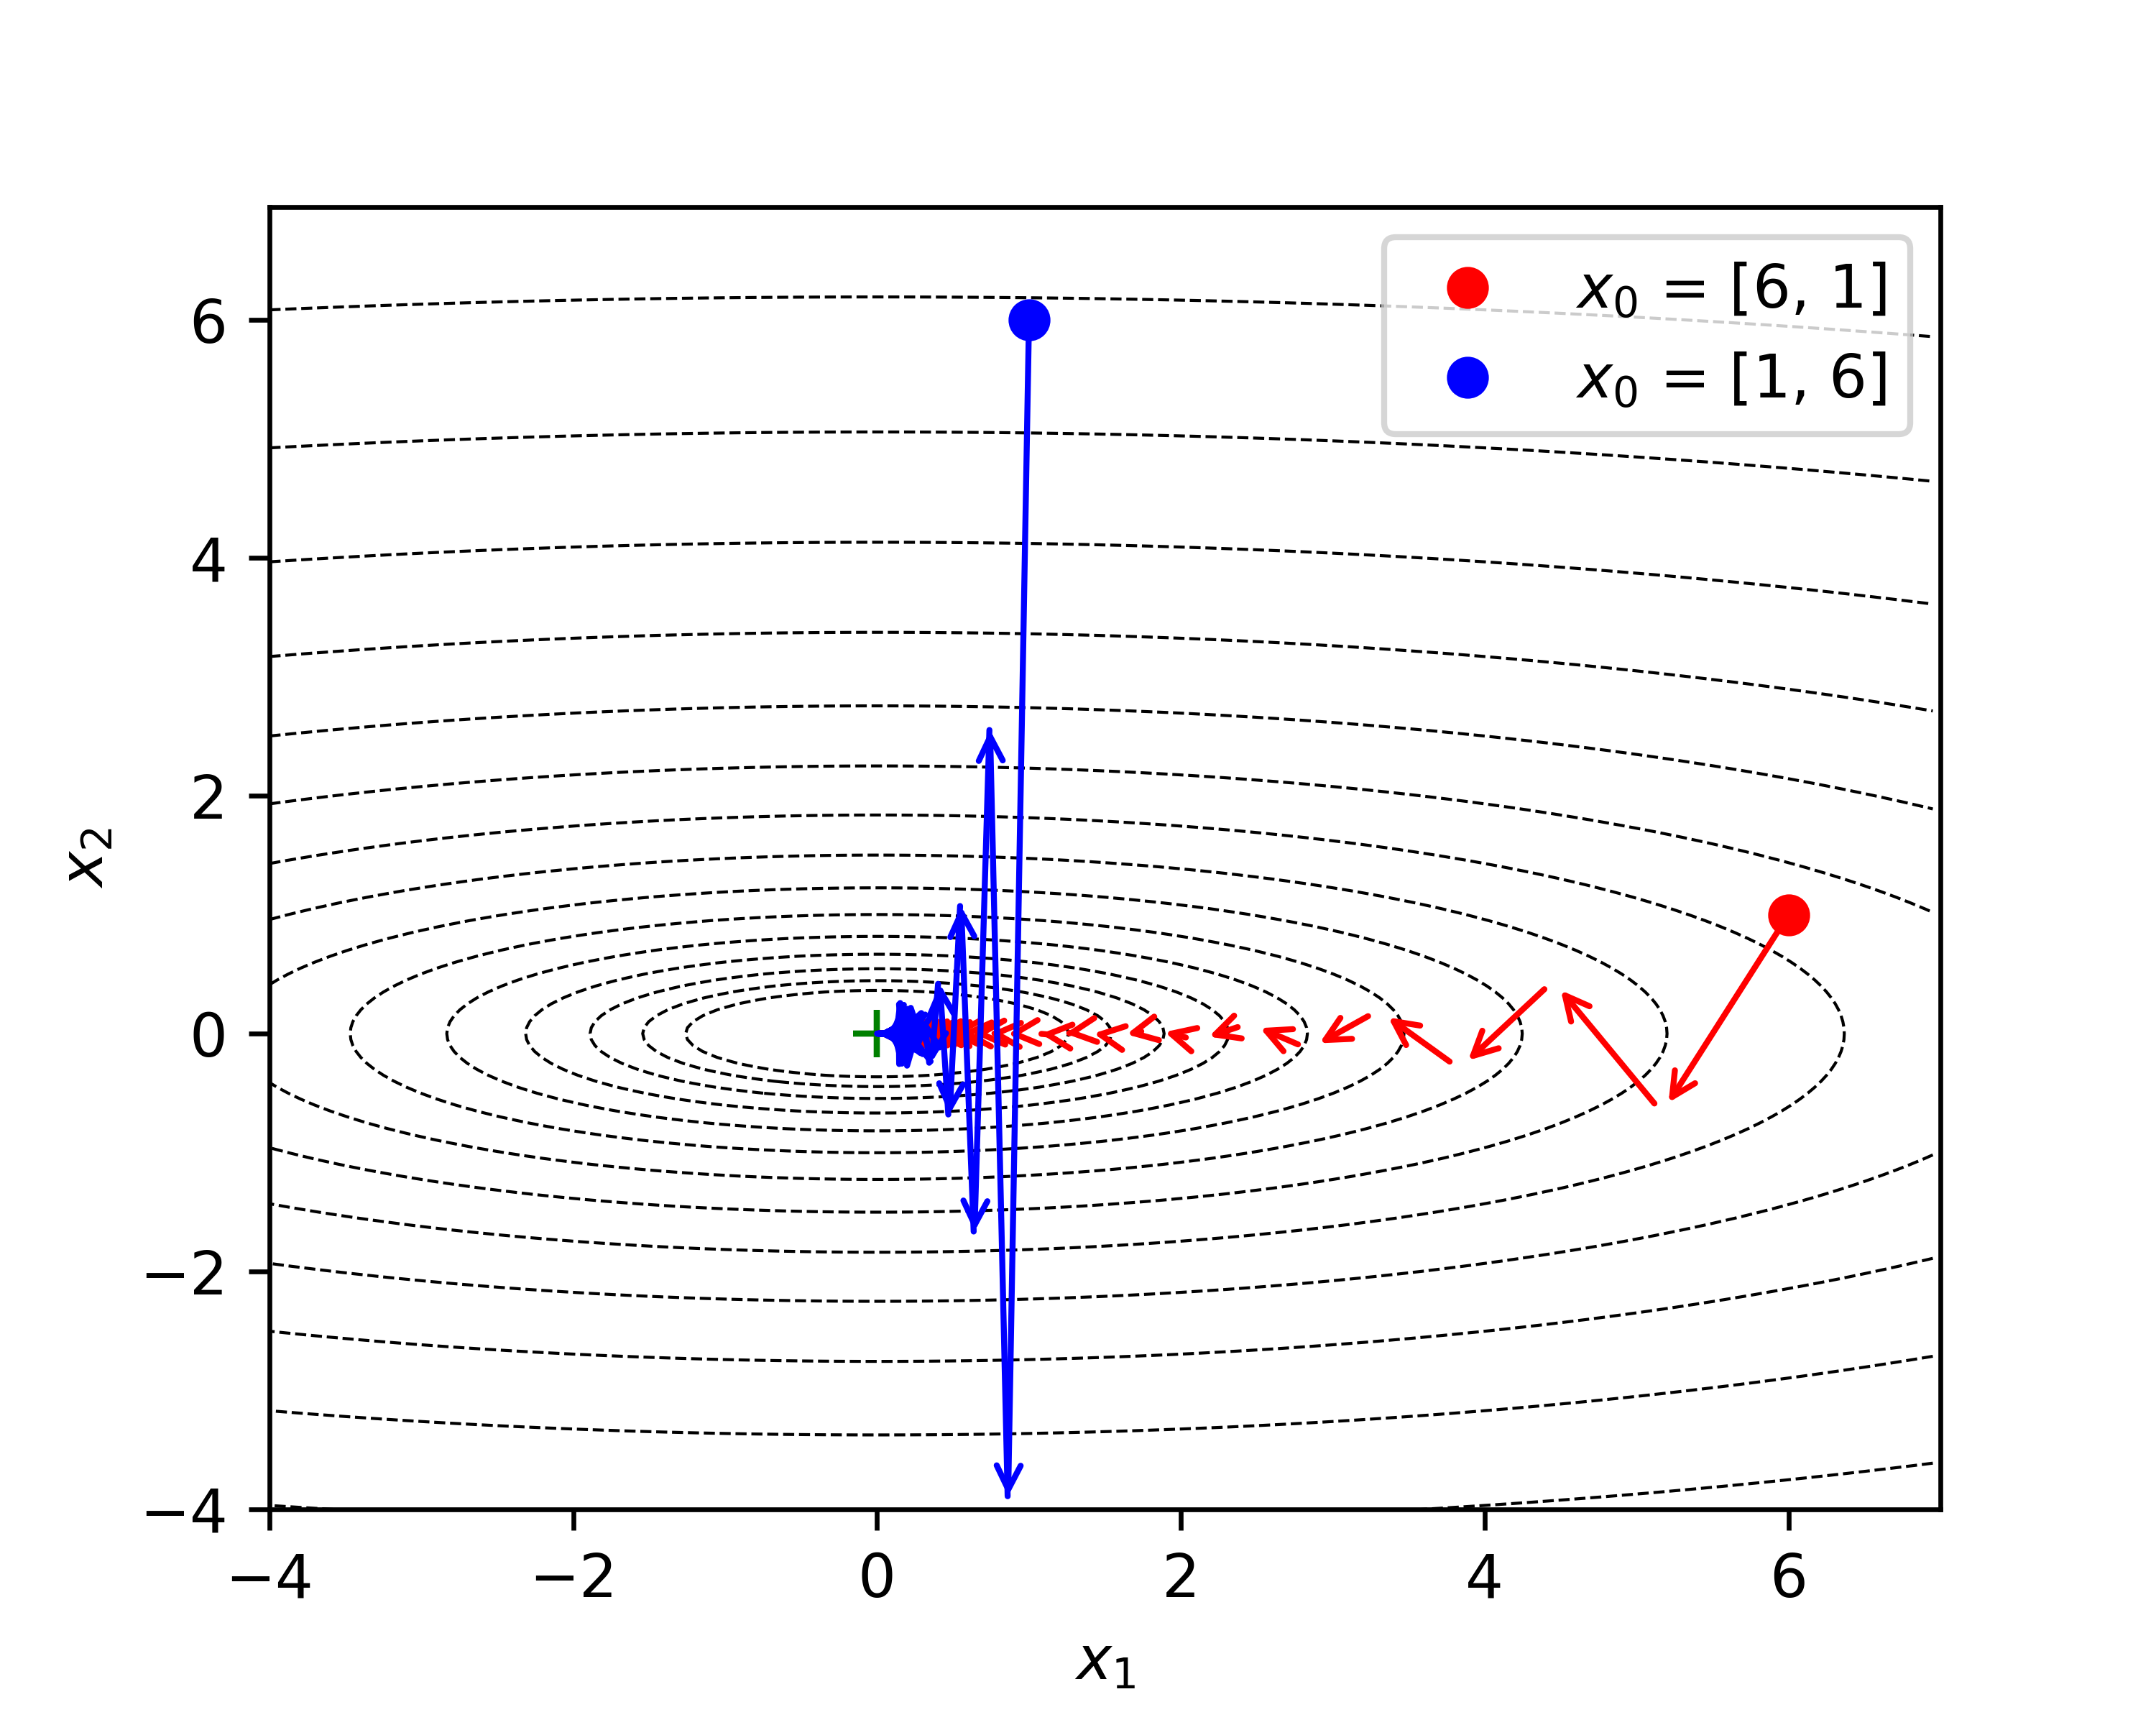
\includegraphics[width=\textwidth]{figs/large_step.png}
        \caption{Steepest descent, large fixed step size.}
        \label{fig:graddesc_large}
    \end{subfigure}
    \begin{subfigure}[b]{0.46\linewidth}
        \centering
        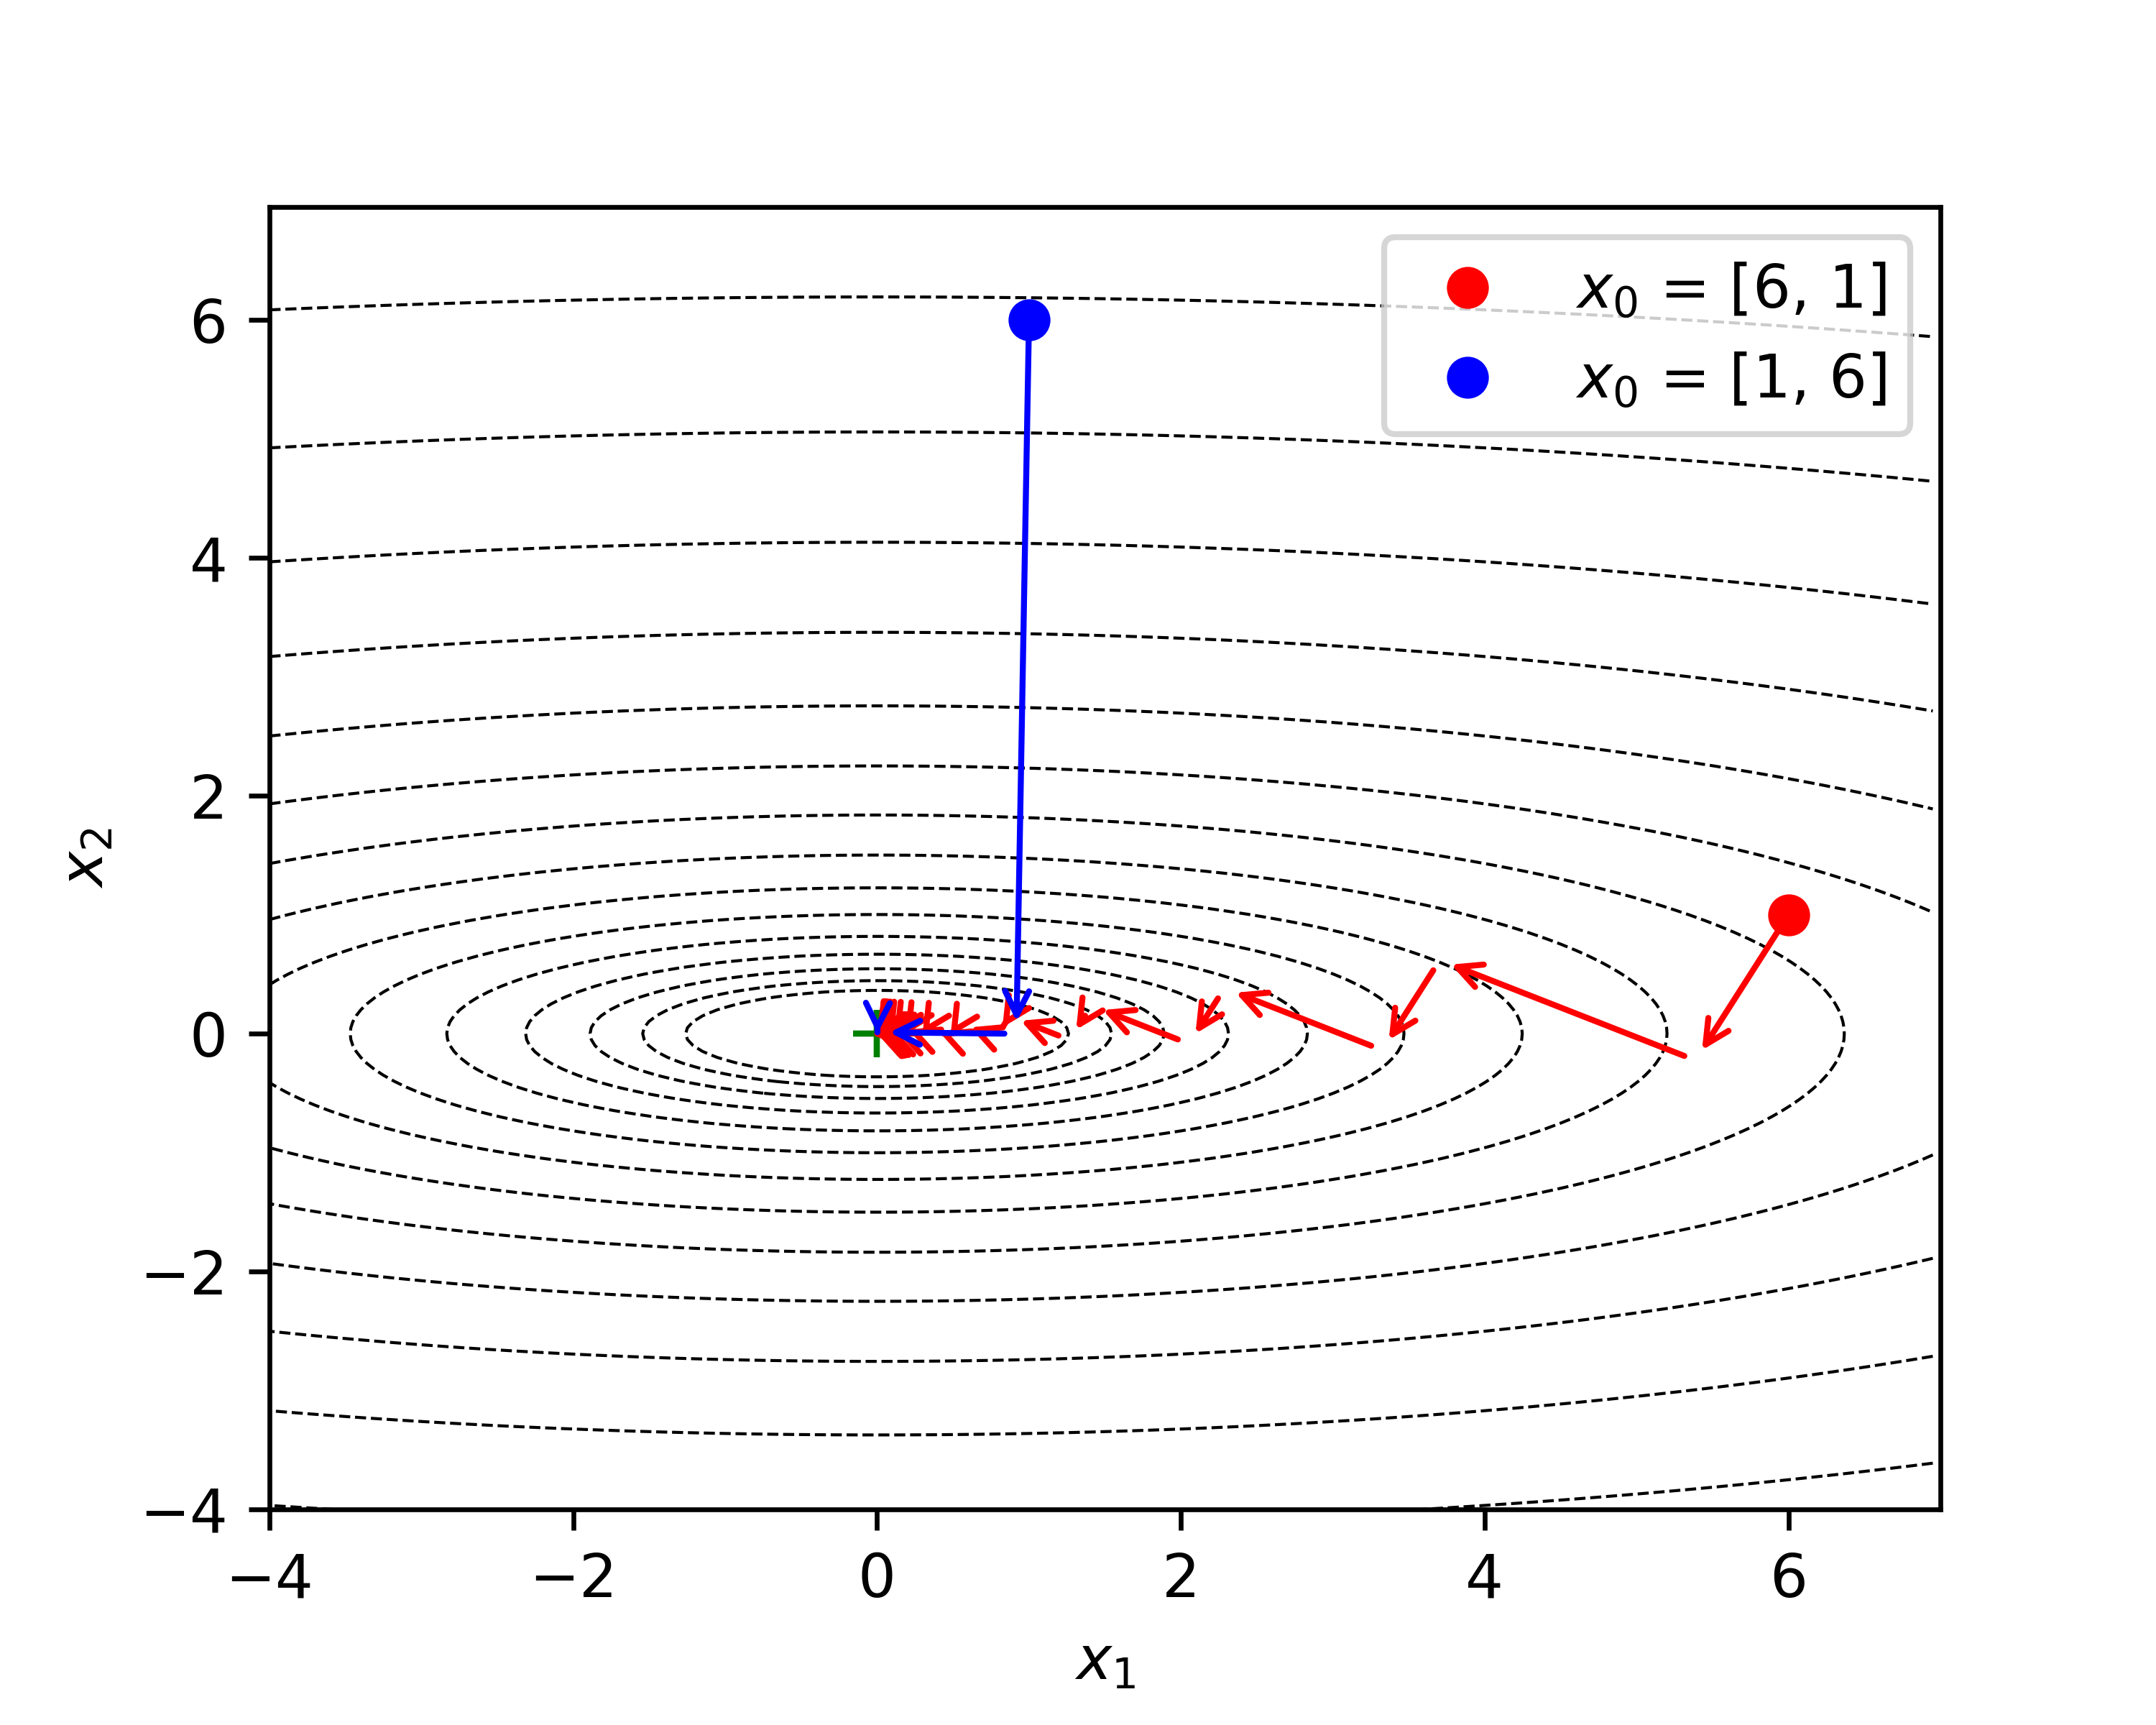
\includegraphics[width=\textwidth]{figs/linesearch.png}
        \caption{Steepest descent, step size chosen via line search.}
        \label{fig:graddesc_line}
    \end{subfigure}%
    \begin{subfigure}[b]{0.46\linewidth}
        \centering
        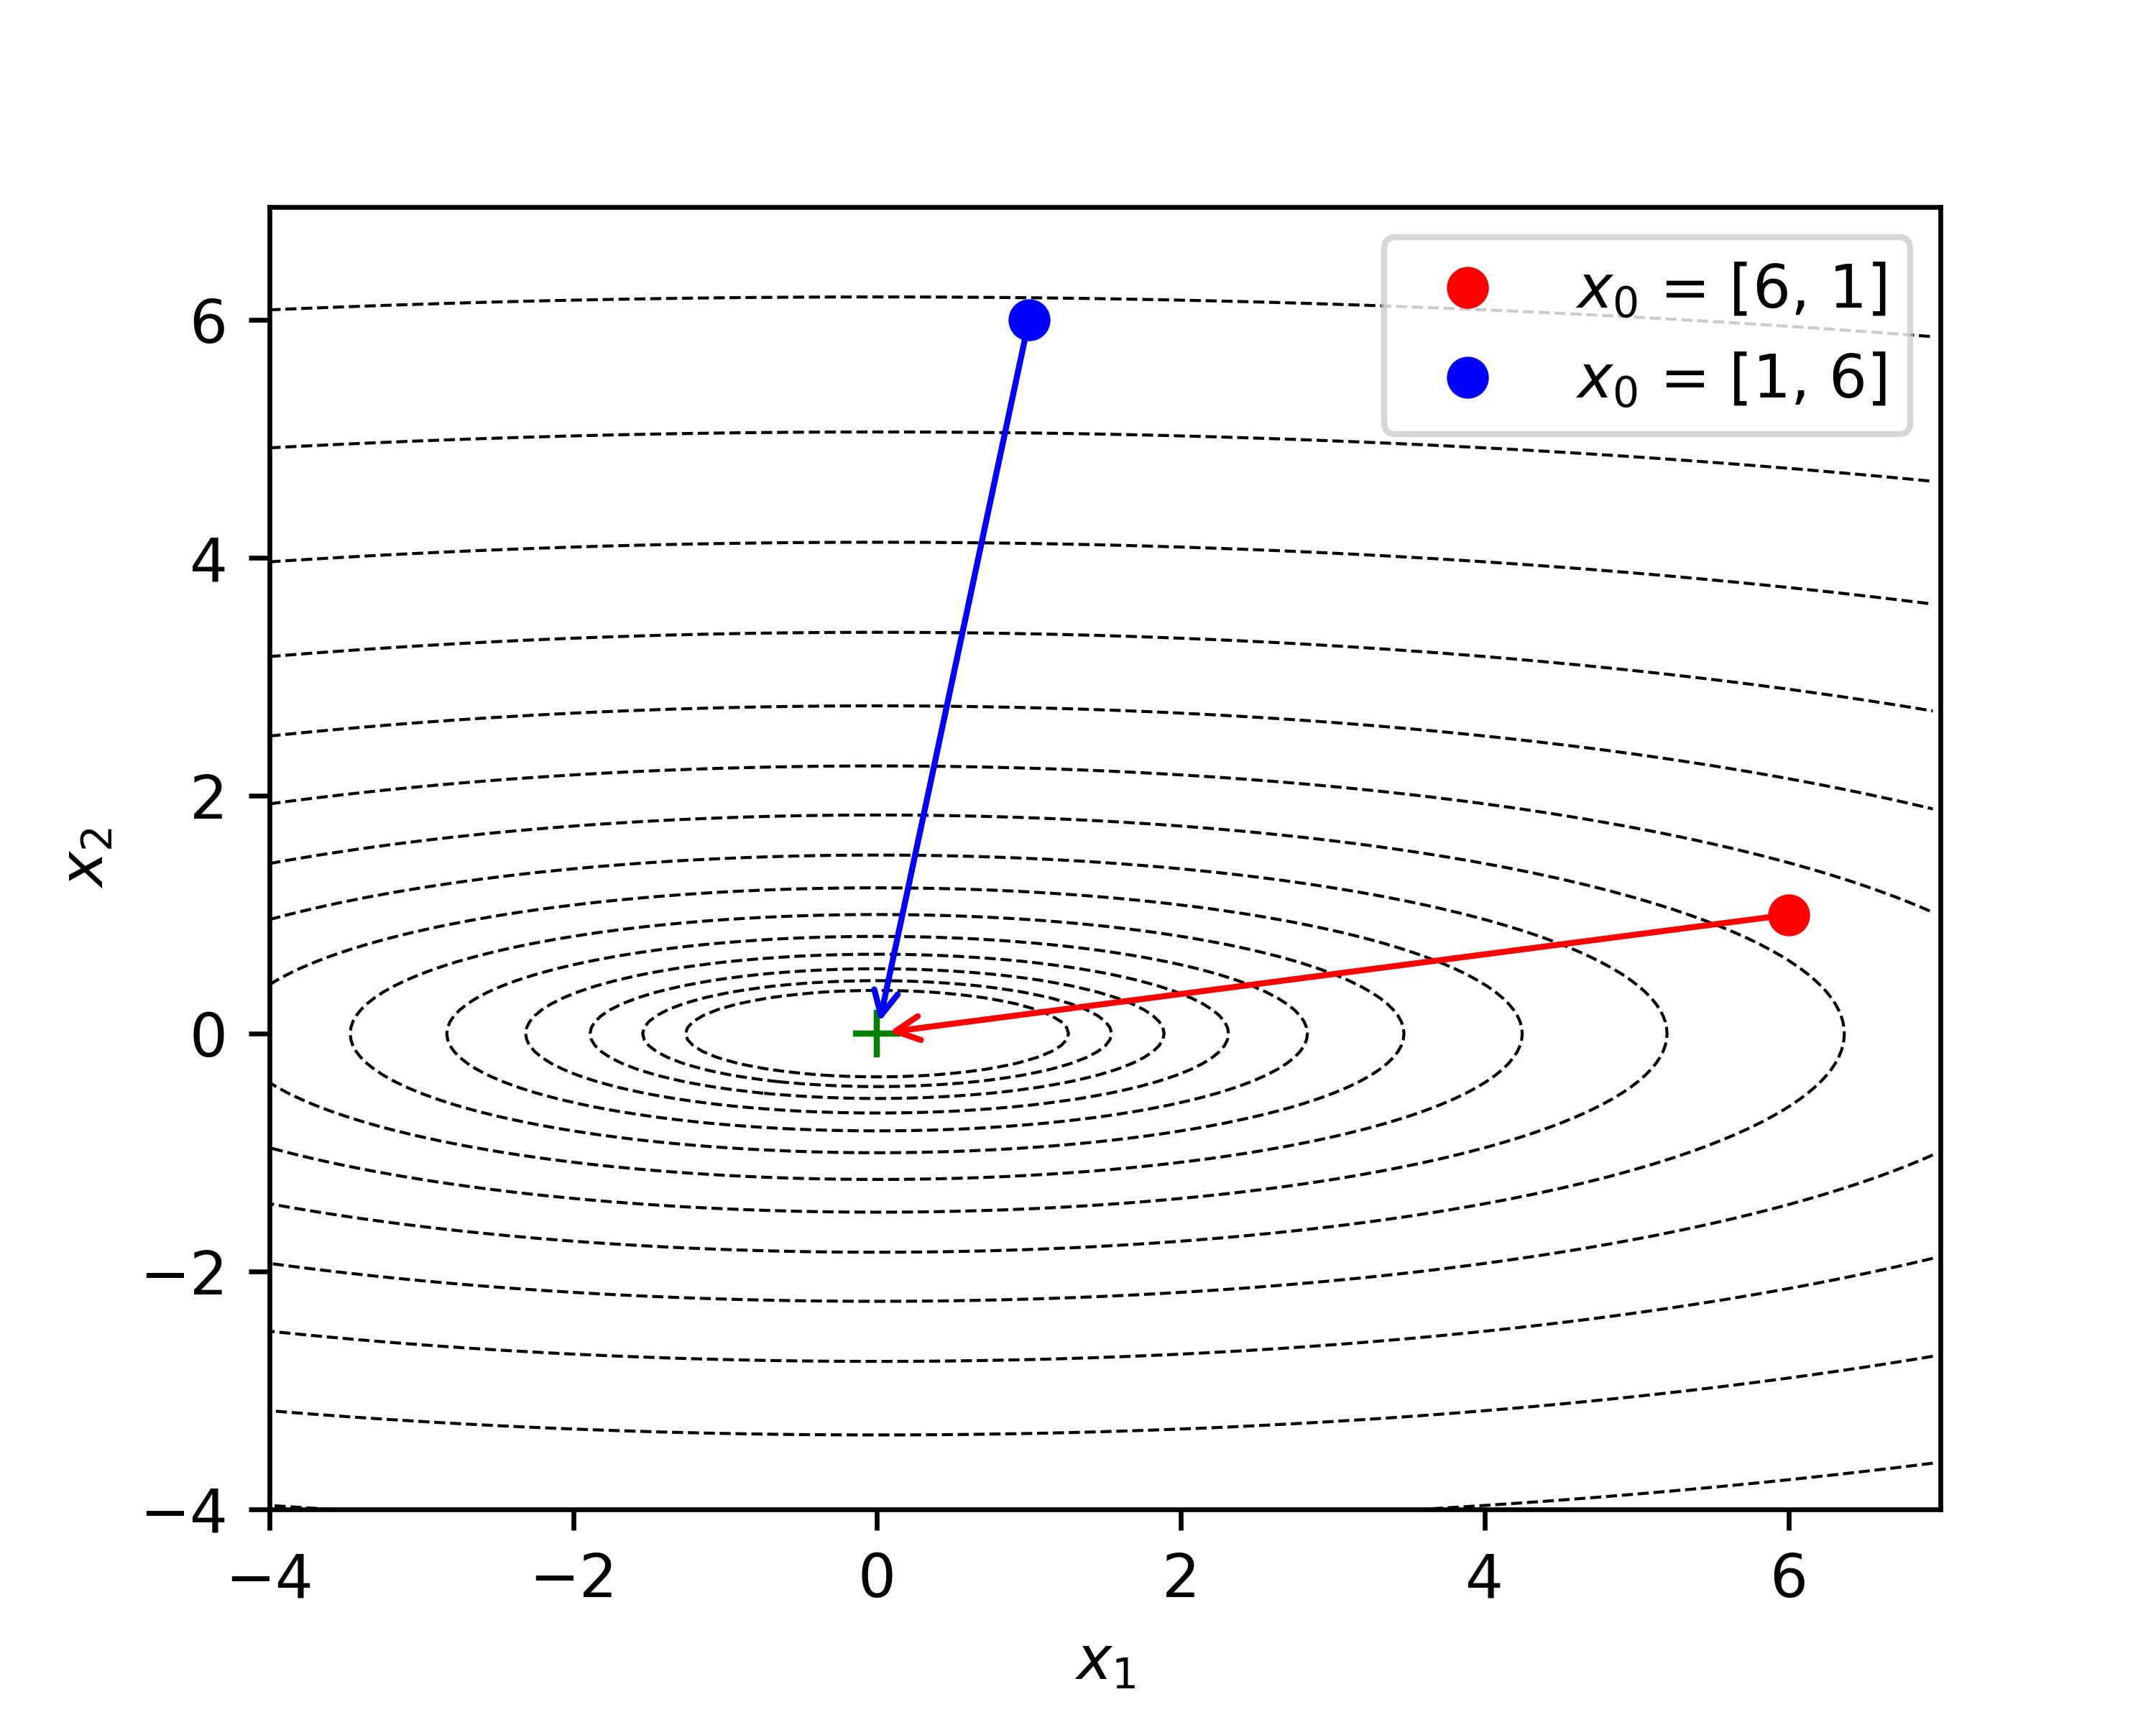
\includegraphics[width=\textwidth]{figs/newtonmethod.png}
        \caption{Newton's method. Note that the method converges in one step.}
        \label{fig:graddesc_newton}
    \end{subfigure}
    \caption{Comparison of steepest descent methods with various step sizes, and Newton's method, on the same quadratic cost function.}
    \label{fig:gradient_descent}
\end{figure}

\paragraph{Newton's Method, $D^k = (\nabla^2 f(\bm{x}^k))^{-1}$.} The underlying idea of this approach is to at each iteration, minimize the quadratic approximation of $f$ around $\bm{x}^k$,
\begin{equation}
    f^k(\bm{x}) = f(\bm{x}^k) + \nabla f(\bm{x}^k)^T (\bm{x} - \bm{x}^k) + \frac{1}{2} (\bm{x} - \bm{x}^k)^T \nabla^2 f(\bm{x}^k) (\bm{x} - \bm{x}^k).
\end{equation}
Setting the derivative of this to zero, we obtain 
\begin{equation}
    \nabla f(\bm{x}^k) + \nabla^2 f(\bm{x}^k) (\bm{x} - \bm{x}^k) = 0
\end{equation}
and thus, by setting $\bm{x}^{k+1}$ to be the $\bm{x}$ that satisfies the above, we get the
\begin{equation}
    \bm{x}^{k+1} = \bm{x}^k - (\nabla^2 f(\bm{x}^k))^{-1} \nabla f(\bm{x}^k)
\end{equation}
or more generally, 
\begin{equation}
    \bm{x}^{k+1} = \bm{x}^k - \alpha (\nabla^2 f(\bm{x}^k))^{-1} \nabla f(\bm{x}^k).
\end{equation}
Note that this update is only valid for $\nabla^2 f(\bm{x}^k) > 0$. When this condition doesn't hold, $\bm{x}^{k+1}$ is not a minimizer of the second order approximation (as a result of the SOCs). See figure \ref{fig:graddesc_newton} for an example where Newton's method converges in one step, as a result of the cost function being quadratic. 

\paragraph{Diagonally scaled steepest descent, $D^k = \textrm{diag}(d_1^k, \ldots, d_n^k)$.} Have $d_i^k >0 \forall i$. A popular choice is 
\begin{equation}
    d_i^k = \left( \frac{\partial^2 f(\bm{x}^k)}{\partial x_i^2} \right)^{-1}
\end{equation}
which is a diagonal approximation of the Hessian. 

\paragraph{Modified Newton's method, $D^k = (\nabla^2 f(\bm{x}^0))^{-1}$.} Requires $\nabla^2 f(\bm{x}^0) > 0$. For cases in which one expects $\nabla^2 f(\bm{x}^0) \approx \nabla^2 f(\bm{x}^k)$, this removes having to compute the Hessian at each step. 

In addition to choosing the descent direction, there also exist a variety of methods to choose the step size $\alpha$. A computationally intensive but efficient (in terms of the number of steps taken) is using a minimization rule of the form 
\begin{equation}
\alpha^k = \argmin_{\alpha\geq 0} f(\bm{x}^k + \alpha \bm{d}^k)  
\end{equation}
which is usually solved via line search (figure \ref{fig:graddesc_line}). Alternative approaches include a limited minimization rule, in which you constrain $\alpha^k \in [0,s]$ during the line search, or simpler approach such as a constant step size (which may not guarantee convergence), or a diminishing scheduled step size. In this last case, schedules are typically chosen such that $\alpha^k \to 0$ as $k \to \infty$, while $\sum_{k=0}^\infty \alpha^k = +\infty$.

\subsection{Constrained Nonlinear Optimization}

In this section we will address the general constrained nonlinear optimization problem,
\begin{equation*}
\begin{aligned}
& \underset{\bm{x} \in \mathcal{X}}{\min}
& & f(\bm{x})
\end{aligned}
\end{equation*}
which may equivalently be written
\begin{equation*}
\begin{aligned}
& \underset{\bm{x}}{\min}
& & f(\bm{x})\\
& \textrm{s.t.} & & \bm{x} \in \mathcal{X}
\end{aligned}
\end{equation*}
where the set $\mathcal{X}$ is usually specified in terms of equality and inequality constraints. To operate within this problem structure, we will develop a set of optimality conditions involving auxiliary variables called \textit{Lagrange multipliers}. 

\subsubsection{Equality Constrained Optimization}

We will first look at optimization with equality constraints of the form 
\begin{equation*}
\begin{aligned}
& \underset{\bm{x}}{\min}
& & f(\bm{x})\\
& \textrm{s.t.} & & h_i(\bm{x}) = 0, \quad i = 1, \ldots, m
\end{aligned}
\end{equation*}
where $f:\R^n \to \R$, $h_i:\R^n \to \R$ are $C^1$. We will write $\bm{h} = [h_1,\ldots, h_m ]^T$. For a given local minimum $\bm{x}^*$, there exist scalars $\lambda_1, \ldots, \lambda_m$ called Lagrange multipliers such that 
\begin{equation}
    \nabla f(\bm{x}^*) + \sum^m_{i=1} \lambda_i \nabla h_i(\bm{x}^*) = 0.
\end{equation}
There are several possible interpretations for Lagrange multipliers. First, note that the cost gradient $f(\bm{x}^*)$ is in the subspace spanned by the constraint gradients at $\bm{x}^*$. Equivalently, $f(\bm{x}^*)$ is orthogonal to the subspace of first order feasible variations 
\begin{equation}
    V(\bm{x}^*) = \{\Delta \bm{x} \mid \nabla h_i(\bm{x}^*)^T \Delta \bm{x}, i=1,\ldots,m\}.
\end{equation}
This subspace is the space of variations $\Delta \bm{x}$ for which $\bm{x} = \bm{x}^* + \Delta \bm{x}$ satisfies the constraint $\bm{h}(\bm{x}) = 0$ up to first order. Therefore, at a local minimum, the first order cost variation $\nabla f(\bm{x}^*)^T \Delta \bm{x}$ is zero for all variations $\Delta \bm{x}$ in this space. 

Given this informal understanding, we may now precisely state the necessary conditions for optimality in constrained optimization. 

\begin{theorem}[NOC for equality constrained optimization]
\label{thm:eq_con_NOC}
Let $\bm{x}^*$ be a local minimum of $f$ subject to $\bm{h}(\bm{x}) = 0$, and assume that the constraint gradients $\nabla h_1(\bm{x}^*),\ldots,\nabla h_m(\bm{x}^*)$ are linearly independent. Then there exists a unique vector $\bm{\lambda}^* = [\lambda_1^*,\ldots,\lambda_m^*]^T$ called a Lagrange multiplier vector, such that
\begin{equation}
    \nabla f(\bm{x}^*) + \sum^m_{i=1} \lambda_i \nabla h_i(\bm{x}^*) = 0.
\end{equation}
If in addition $f$ and $\bm{h}$ are $C^2$, we have 
\begin{equation}
    \bm{y}^T (\nabla^2 f(\bm{x}^*) + \sum^m_{i=1} \lambda_i \nabla^2 h_i(\bm{x}^*)) \bm{y} \geq 0, \quad \forall \bm{y} \in V(\bm{x}^*) 
\end{equation}
where
\begin{equation}
    V(\bm{x}^*) = \{\bm{y} \mid \nabla h_i(\bm{x}^*)^T \bm{y} = 0, i=0,\ldots,m\}.
\end{equation}
\end{theorem}

\begin{proof}
See \cite{bertsekas2016nonlinear} Section 3.1.1 and 3.1.2.
\end{proof}

We will sketch two possible proofs for the NOC for equality constrained optimization. 

\paragraph{Penalty approach.} This approach relies on adding a to the cost function a large penalty term for constraint violation. This is the same approach that will be used in proving the necessary conditions for inequality constrained optimization, and is the basis of a variety of practical numerical algorithms. 

\paragraph{Elimination approach.} This approach views the constraints as a system of $m$ equations with $n$ unknowns, for which $m$ variables can be expressed in terms of the remaining $m-n$ variables. This reduces the problem to an unconstrained optimization problem. 

Note that in theorem \ref{thm:eq_con_NOC}, we assumed the gradients of the constraint functions were linearly independent. A feasible vector for which this holds is called \textit{regular}. If this condition is violated, a Lagrange multiplier for a local minimum may not exist. 

For convenience, we will write the necessary conditions in terms of the Lagrangian function $L:\R^{m+n} \to \R$,
\begin{equation}
    L(\bm{x},\bm{\lambda}) = f(\bm{x}) + \sum^m_{i=1} \lambda_i h_i(\bm{x}).
\end{equation}
This function allows the NOC conditions to be succinctly stated as 
\begin{align}
    \nabla_{\bm{x}} L(\bm{x}^*,\bm{\lambda}^*) &= 0\\
    \nabla_{\bm{\lambda}} L(\bm{x}^*,\bm{\lambda}^*) &= 0\\
    \bm{y}^T \nabla^2_{\bm{xx}} L(\bm{x}^*,\bm{\lambda}^*) \bm{y} &\geq 0, \quad \forall \bm{y} \in V(\bm{x}^*).
\end{align}
which form a system of $n+m$ equations with $n+m$ unknowns. Given this notation, we can state the sufficient conditions. 

\begin{theorem}[SOC for equality constrained optimization]
Assume that $f$ and $\bm{h}$ are $C^2$ and let $\bm{x}^* \in \R^n$ and $\bm{\lambda}^* \in \R^m$ satisfy
\begin{align}
    \nabla_{\bm{x}} L(\bm{x}^*,\bm{\lambda}^*) &= 0\\
    \nabla_{\bm{\lambda}} L(\bm{x}^*,\bm{\lambda}^*) &= 0\\
    \bm{y}^T \nabla^2_{\bm{xx}} L(\bm{x}^*,\bm{\lambda}^*) \bm{y} &> 0, \quad \forall \bm{y} \neq 0, \bm{y} \in V(\bm{x}^*).
\end{align}
\end{theorem}

\begin{proof}
See \cite{bertsekas2016nonlinear} Section 3.2.
\end{proof}
Note that the SOC does not include regularity of $\bm{x}^*$. 

\subsubsection{Inequality Constrained Optimization}

We will now address the general case, including inequality constraints,
\begin{equation*}
\begin{aligned}
& \underset{\bm{x}}{\min}
& & f(\bm{x})\\
& \textrm{s.t.} & & h_i(\bm{x}) = 0, \quad i = 0, \ldots, m\\
& & & g_j(\bm{x}) \leq 0, \quad j = 0, \ldots, r
\end{aligned}
\end{equation*}
where $f,h_i,g_i$ are $C^1$. The key intuition for the case of  inequality constraints is based on realizing that for any feasible point, some subset of the constraints will be active (for which $g_j(\bm{x}) = 0$), while the complement of this set will be inactive. We define the active set of inequality constraints, which we denote 
\begin{equation}
    A(\bm{x}) = \{j \mid g_j(\bm{x} = 0\}.
\end{equation}
A constraint is active at $\bm{x}$ if it is in $A(\bm{x})$, otherwise it is inactive. Note that if $\bm{x}^*$i is a local minimum of the inequality constrained problem, then $\bm{x}^*$ is a local minimum of the identical problem with the inactive constraints removed. Moreover, at this local minimum, the constraints may be treated as equality constraints. Thus, if $\bm{x}^*$ is regular, there exists Lagrange multipliers $\lambda_1^*, \ldots, \lambda_m^*$ and $\mu_j^*, j \in A(\bm{x}^*)$ such that 
\begin{equation}
\nabla f(\bm{x}^*) + \sum^m_{i=1} \lambda_i \nabla h_i(\bm{x}^*) + \sum_{j \in A(\bm{x}^*)} \mu_j^* \nabla g_j(\bm{x}^*)= 0.    
\end{equation}
We will define the Lagrangian
\begin{equation}
    L(\bm{x},\bm{\lambda}, \bm{\mu}) = f(\bm{x}) + \sum^m_{i=1} \lambda_i h_i(\bm{x}) + \sum_{j =1}^r \mu_j^*  g_j(\bm{x}^*),
\end{equation}
which we will use to state the necessary and sufficient conditions. 

\begin{theorem}[Karush-Kuhn-Tucker NOC]
Let $\bm{x}^*$ be a local minimum for the inquality constrained problem where $f, h_i, g_j$ are $C^1$ and assume $\bm{x}^*$ is regular (equality and active inequality constraint gradients are linearly independent). Then, there exists unique Lagrange multiplier vectors $\bm{\lambda}^*$ and $\bm{\mu}^*$ such that
\begin{align}
    \nabla_{\bm{x}} L(\bm{x}^*,\bm{\lambda}^*, \bm{\mu}^*) &= 0\\
    \bm{\mu} &\geq 0\\
    \mu_j^* &= 0, \quad \forall j \notin A(\bm{x}^*)
\end{align}
If in addition, $f,\bm{h},\bm{g}$ are $C^2$, we have 
\begin{equation}
    \bm{y}^T \nabla^2_{\bm{xx}} L(\bm{x}^*,\bm{\lambda}^*, \bm{\mu}^*) \bm{y} \geq 0 
\end{equation}
for all $\bm{y}$ such that 
\begin{align}
    \nabla h_i(\bm{x}^*)^T \bm{y} &=0, \quad i = 1, \ldots, m\\
    \nabla g_j(\bm{x}^*)^T \bm{y} &=0, \quad j \in A(\bm{x}^*)
\end{align}
\end{theorem}

\begin{proof}
See \cite{bertsekas2016nonlinear} Section 3.3.1.
\end{proof}

The SOC are obtained similarly to the equality constrained case. 

% should add in statement of KKT SOC for completeness

% should we add section on convex optimization from recitation?

\subsection{Further Reading}

In this section we have addressed the necessary and sufficient conditions for constrained and unconstrained nonlinear optimization. This section is based heavily on \cite{bertsekas2016nonlinear}, and we refer the reader to this book for further details. We have avoided discussing linear programming, which is itself a large topic of study, about which many books have been written (we refer the reader to \cite{bertsimas1997introduction} as a good reference on the subject). 

Convex optimization has become a powerful and widespread tool in modern optimal control. While we have only addressed it briefly here, \cite{boyd2004convex} offers a fairly comprehensive treatment of the theory and practice of convex optimization. For a succinct overview with a focus on machine learning, we refer the reader to \cite{kolter2008convex}.
